\documentclass[aspectratio=43]{beamer}
\usepackage[latin1]{inputenc}
\usepackage{amsmath}
\usepackage{amsfonts}
\usepackage{amssymb}
\usepackage{makeidx}
\usepackage{graphicx}
\usepackage{array}
\usepackage{braket}

% Customization
\mode<presentation>{
\usetheme{CambridgeUS}
\usecolortheme{dolphin}
\setbeamertemplate{navigation symbols}{}
}

%\setbeamertemplate{footline}[frame number]

% Title and author
\title[Quantum coherent phenomena]{Quantum coherent phenomena}
\author{\textbf {Jes\'us Urtasun Elizari}}
%\institute{\textbf {University of Milan}}
\date{Milan, October 2020}

\begin{document}

% Front slide
\begin{frame}

	%\maketitle
	\vspace{1.0 cm}
	
	\center{\color{blue}Two-mode squeezed states in cavity optomechanics\\ via engineering of a single reservoir}
	
	\vspace{0.25 cm}
	\center{PhD course - Quantum coherent phenomena\\ Milan, October 2020}

	\begin{figure}
		\minipage{1\textwidth}
		
\includegraphics[width = 3.0 cm]{plots/logo_unimi.png}
		\hfill
		
\includegraphics[width = 3.0 cm]{plots/logo_infn.png}
		\hfill
		
\includegraphics[width = 3.0 cm]{plots/logo_erc.png}
		\endminipage
	\end{figure}

	\vspace{1.0 cm}

\end{frame}

% Introduction
\begin{frame}

	\frametitle{Outline}
	
	\begin{enumerate}
		\item {\color{blue}System and Hamiltonian}
		\item {\color{blue}Implementation strategies}
		\item {\color{blue}Observable quantities}
		\item {\color{blue}Experimental observability}
		\item {\color{blue}Conclusions}
	\end{enumerate}
	
\end{frame}

% System and Hamiltonian I
\begin{frame}

	\frametitle{Introduction}
	\framesubtitle{System representation}
	
	\begin{itemize}
		\item Two mechanical oscillators with resonance frequencies $\omega_{a}, \omega_{b}$
		\item Dispersively coupled with rates $g_{a}, g_{b}$ to a common cavity $\omega_{c}$
		\item Apply radiation pressure forces inside the cavity leading to generate entangled motion of the mirrors
	\end{itemize}

		\begin{figure}
			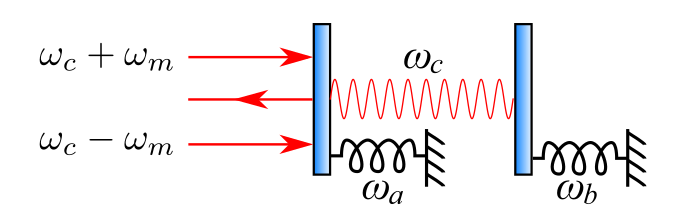
\includegraphics[width = 8 cm]{plots/plot_system.png}
		\end{figure}	

\end{frame}

% System and Hamiltonian II
\begin{frame}
	
	\frametitle{Introduction}
	\framesubtitle{System and Hamiltonian}
	
	Quantum optomechanics $\longrightarrow$ describing optical and mechanical modes with same formalism 
	\begin{figure}
		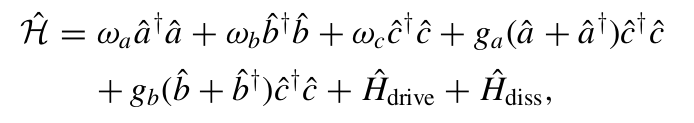
\includegraphics[width = 8 cm]{plots/hamiltonian_1.png}
	\end{figure}
	
	under usual approximations, obtain the master equation 
	\begin{figure}
		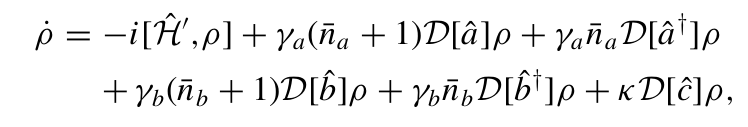
\includegraphics[width = 8 cm]{plots/master_eq_1.png}
	\end{figure}

	being $\mathcal{H}' = \mathcal{H} - \mathcal{H}_{\textrm{diss}}$, and $\mathcal{D}[\hat{c}]$ the dispersive superoperator\\
	Only dissipation term for $\hat{c} \longrightarrow$ {\color{blue}Assuming zero thermal occupation}
	
\end{frame}

% Reservoir engineering I
\begin{frame}
	
	\frametitle{Reservoir engineering strategies}
	\framesubtitle{Bogoliubov operators}
	
	Define the {\color{blue}Bogoliuov} mechanical modes in terms of the modes $\hat{a}, \hat{b}$
	\begin{figure}
		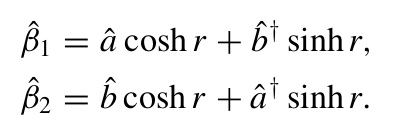
\includegraphics[width = 4.5 cm]{plots/bogoliubov_1.png}
	\end{figure}	

	Where r is the {\color{blue}squeezing parameter}.
	
	\vspace{0.5 cm}

	Work in rotating frame with respect to the Hamiltonian:
	\begin{figure}
		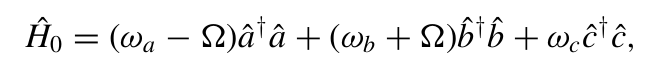
\includegraphics[width = 8 cm]{plots/hamiltonian_2.png}
	\end{figure}

\end{frame}

% Reservoir engineering VII
\begin{frame}
	
	\frametitle{Reservoir engineering strategies}
	\framesubtitle{Hamiltonian}
	
	Hamiltonian in terms of the Bogoliubov modes
	\begin{figure}
		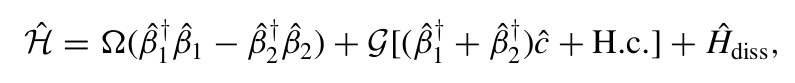
\includegraphics[width = 8.5 cm]{plots/hamiltonian_3.png}
	\end{figure}	
	
	where $\Omega$ is the effective oscillation frequency and $\mathcal{G}$ an effective optomechanical coupling.
	
	\vspace{0.5 cm}
	
	Written in terms of the original operators,
	\begin{figure}
		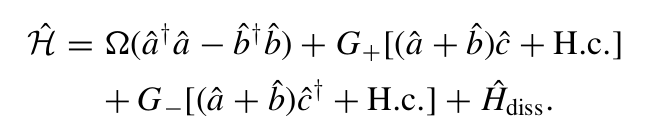
\includegraphics[width = 7.5 cm]{plots/hamiltonian_4.png}
	\end{figure}
	
	with couplings related by $\mathcal{G} \equiv \sqrt{G_{-}^{2} - G_{+}^{2}}$ and ${\color{blue}\tanh r \equiv G_{+}/G_{-}}$

\end{frame}

% Reservoir engineering III
\begin{frame}
	
	\frametitle{Reservoir engineering strategies}
	\framesubtitle{2-mode squeezed state}
	
	Define the {\color{blue}2-mode squeezed state} as $\ket{r}_{2} = \hat{S}_{2}(r) \ket{0,0}$, being the squeezing operator
	\begin{figure}
		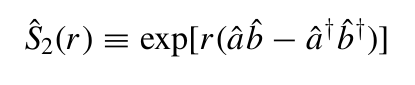
\includegraphics[width = 4.5 cm]{plots/2_squeezed_mode.png}
	\end{figure}	

	such that $[\hat{S}_{2}(r) \hat{a} \hat{S}_{2}^{\dagger}(r)]\ket{r}_{2} = [\hat{S}_{2}(r) \hat{b} \hat{S}_{2}^{\dagger}(r)]\ket{r}_{2} = 0$\\
	
	\vspace{0.5cm}
	
	Therefore, $\hat{\beta}_{1} = \hat{S}_{2}(r) \hat{a} \hat{S}_{2}^{\dagger}(r)$, $\hat{\beta}_{2} = \hat{S}_{2}(r) \hat{b} \hat{S}_{2}^{\dagger}(r)$ and their\\ground state is the two-mode squeezed state with squeezing parameter $r$.

\end{frame}

% Reservoir engineering V
\begin{frame}
	
	\frametitle{Reservoir engineering strategies}
	\framesubtitle{Note on Quantum Optomechanics}
	
	Linearized Hamiltonian with 2-tone laser with amplitudes $\alpha_{+}$ and $\alpha_{-}$
	
	\begin{equation}
	\mathcal{H} = \hbar \textrm{g}_{+} \; (a^{\dagger}b^{\dagger} + ab) + \hbar \textrm{g}_{-} \; (a^{\dagger}b + ab^{\dagger}) \nonumber
	\end{equation}
	
	being $g_{\pm} = g_{0} \alpha_{\pm}$\\

	\vspace{0.5 cm}
	
	Study different cases
	
	\begin{itemize}
		\item $g_{-} = 0 \longrightarrow$ Sideband blue $\mathcal{H} = \hbar \textrm{g} \; (a^{\dagger}b^{\dagger} + ab)$ "2 - mode squeezing"
		\item $g_{+} = 0 \longrightarrow$ Sideband red $\mathcal{H} = \hbar \textrm{g} \; (a^{\dagger}b + ab^{\dagger})$ {\color{blue}"beam - splitter"}
		\item $g_{-} = g_{+} = g \longrightarrow \mathcal{H} = \hbar \textrm{g} \; (a + a^{\dagger})(b + b^{\dagger})$ "back-action evading"
	\end{itemize}	

\end{frame}

% Implementation I
\begin{frame}

	\frametitle{Implementation}
	\framesubtitle{Different cases}
	
	\begin{figure}
		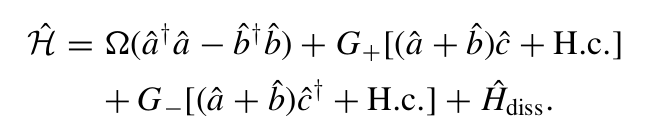
\includegraphics[width = 7.5 cm]{plots/hamiltonian_4.png}
	\end{figure}
	
	already implemented in conventional optomechanical setups.
	
	\vspace{0.5 cm}

	Different cases depending on the optomechanical couplings relation:

	\begin{itemize}
		\item Two-tone driving $(g_{a} = g_{b}) \longrightarrow$ two cavity drives are required 
		\item Four-tone driving $(g_{a} \neq g_{b}) \longrightarrow$ four cavity drives are required 
		\item Case similar $(g_{a} \sim g_{b}) \longrightarrow$ approximate with two cavity drives
	\end{itemize}	

\end{frame}

% Implementation - 2 tone driving
\begin{frame}

	\frametitle{Implementation}
	\framesubtitle{2 - tone driving $(g_{a} = g_{b})$}
	
	Driving tones at $\omega_{c} \pm \omega_{m}$ being  $\omega_{m} = (\omega_{a} + \omega_{b}) / 2$
	
	\begin{figure}
		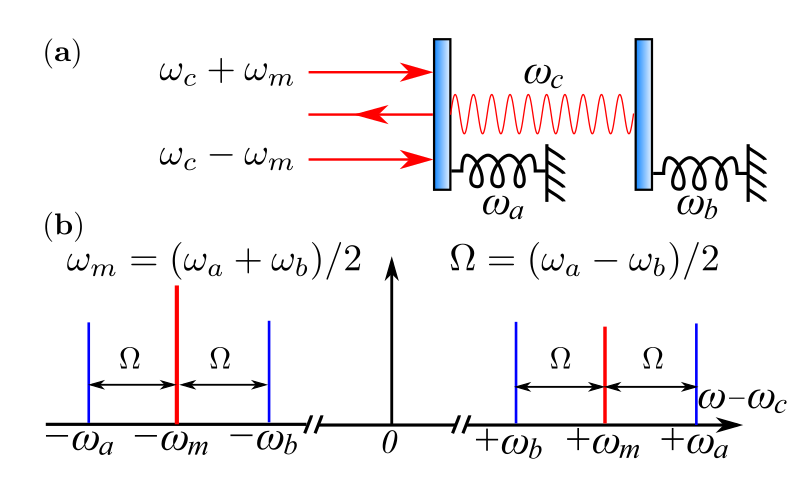
\includegraphics[width = 7 cm]{plots/plot_2_tone.png}
	\end{figure}	

	Apply our drive Hamiltonian

	\begin{figure}
		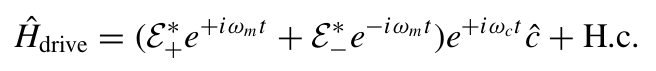
\includegraphics[width = 7 cm]{plots/hamiltonian_2_tone.png}
	\end{figure}

\end{frame}

% Implementation - 2 tone driving
\begin{frame}
	
	\frametitle{Implementation}
	\framesubtitle{2 - tone driving $(g_{a} = g_{b})$}

	Interaction picture with respect to $\hat{\mathcal{H}}_{0} = \omega_{m}(\hat{a}^{\dagger}\hat{a} + \hat{b}^{\dagger}\hat{b}) + \omega_{c}\hat{c}^{\dagger}\hat{c}$ leads back to out desired Hamiltonian
	
	\begin{figure}
		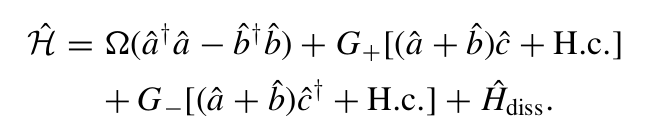
\includegraphics[width = 7 cm]{plots/hamiltonian_4.png}
	\end{figure}
	
	\begin{align}
		\textrm{where} \qquad \Omega &= (\omega_{a} - \omega_{b}) / 2 \nonumber \\
		G_{\pm} &= (g_{a} + g_{b})\bar{c}_{\pm} / 2 \nonumber
	\end{align}
	
	\vspace{0.5 cm}
	
	and $\bar{c}_{\pm}$ are the steady state amplitudes at the sidebands
	\begin{figure}
		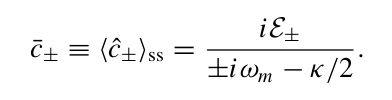
\includegraphics[width = 5 cm]{plots/ss_2_tone.png}
	\end{figure}

\end{frame}

% Implementation - 4 tone driving
\begin{frame}
	
	\frametitle{Implementation}
	\framesubtitle{4 - tone driving $(g_{a} \neq g_{b})$}
	
	Four different sideband processes involved\\
	Driving tones applied with detuning of $\Omega$ from the sidebands at $\omega_{c} \pm (\omega_{a} - \Omega)$ and $\omega_{c} \pm (\omega_{b} + \Omega)$
	
	\begin{figure}
		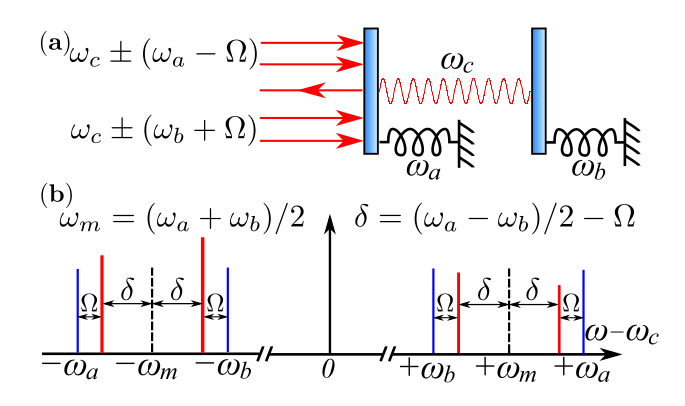
\includegraphics[width = 7 cm]{plots/plot_4_tone.png}
	\end{figure}	

\end{frame}

% Implementation - 4 tone driving
\begin{frame}
	
	\frametitle{Implementation}
	\framesubtitle{4 - tone driving $(g_{a} \neq g_{b})$}
	
	\begin{figure}
		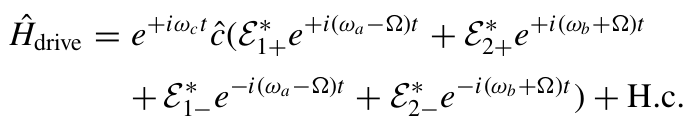
\includegraphics[width = 8 cm]{plots/hamiltonian_4_tone.png}
	\end{figure}

	steady-state amplitudes are now

	\begin{figure}
		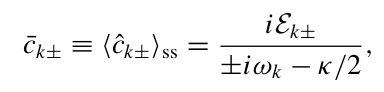
\includegraphics[width = 5 cm]{plots/ss_4_tone.png}
	\end{figure}

	where we introduced notation for the drive detunings

	\begin{align}
	\omega_{1} &= (\omega_{a} - \Omega) \nonumber \\
		\omega_{2} &= (\omega_{b} + \Omega) \nonumber \\
		G_{\pm} &= (g_{a}\bar{c}_{1\pm} + g_{b}\bar{c}_{2\pm}) / 2 \nonumber
	\end{align}

\end{frame}

% Adiabatic limit I
\begin{frame}
	
	\frametitle{Adiabatic limit}
	\framesubtitle{Adiabatically eliminated master equation}
	
	\begin{itemize}
		\item Assume the system responds fast to mechanical motion ($k > \Omega, G_{\pm}$)
		\item Simplify by getting rid of the cavity operator $\hat{c} = -2i\mathcal{G}(\hat{\beta}_{1} + \hat{\beta}_{2})/k$\\
		\item Obtain adiabatically eliminated master equation
	\end{itemize}

	\begin{figure}
		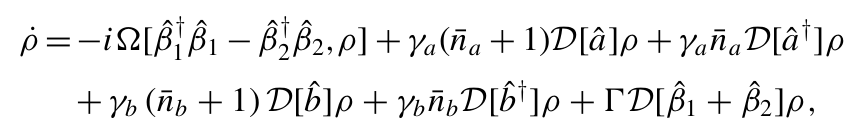
\includegraphics[width = 9 cm]{plots/master_eq_2.png}
	\end{figure}

	with optomechanical damping rate
	\begin{figure}
		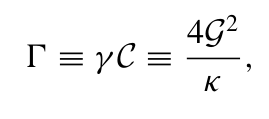
\includegraphics[width = 3 cm]{plots/optomechanic_dumping.png}
	\end{figure}

	easy to obtain steady state, and to measure entanglement and purity.
	 
\end{frame}

% Adiabatic limit II
\begin{frame}
	
	\frametitle{Adiabatic limit}
	\framesubtitle{Entanglement}
	
	Build a way of identify entanglement on a 2-mode system\\
	{\color{blue}Duan criterion} $\longrightarrow$ define collective quadratures
	\begin{figure}
		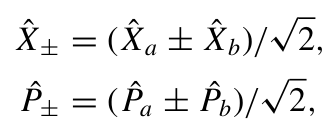
\includegraphics[width = 4 cm]{plots/entanglement_quad.png}
	\end{figure}	
	
	as combination of the usual quadrature modes
	\begin{figure}
		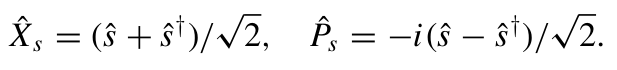
\includegraphics[width = 7 cm]{plots/entanglement_quad_2.png}
	\end{figure}

	Duan inequality states that a state for which
	\begin{figure}
		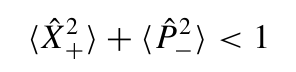
\includegraphics[width = 3.5 cm]{plots/entanglement_duan_criterion.png}
	\end{figure}

	is inseparable $\longrightarrow$ {\color{blue}entangled!}

\end{frame}

% Adiabatic limit III
\begin{frame}

	\frametitle{Adiabatic limit}
	\framesubtitle{Entanglement}
		
	Quadratures can be written as function of the drive asymmetry 
	\begin{figure}
		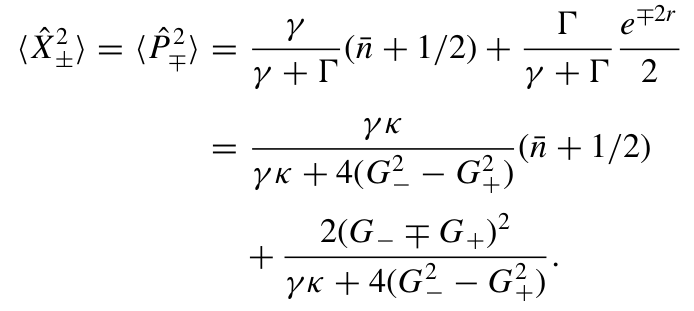
\includegraphics[width = 7.5 cm]{plots/entanglement_quadratures.png}
	\end{figure}

	Use also logarithmic negativity $E_{\mathcal{N}} = \max \{0, -\ln 2\eta \}$,
	with $\eta$ factor in terms of the covariance matrix {\color{blue}*}

\end{frame}

% Adiabatic limit IV
\begin{frame}
	
	\frametitle{Adiabatic limit}
	\framesubtitle{Purity}
	
	Purity defined as trace of the density matrix
	\begin{equation}
		\mu \equiv \textrm{tr}[\rho^{2}] \nonumber
	\end{equation}	
		
	and as function of the covariance matrix {\color{blue}*}
	
	\begin{equation}
		\mu = \frac{1}{4 \sqrt{\det \textbf{V}}} \nonumber
	\end{equation}
	
	\vspace{0.5 cm}
	
	Again, demanding from experimental point of view.
	
\end{frame}

% Adiabatic limit V
\begin{frame}
	
	\frametitle{Adiabatic limit}
	\framesubtitle{Entanglement}
	
	\begin{columns}
		
		\column{0.5\textwidth}
		
		\begin{figure}
			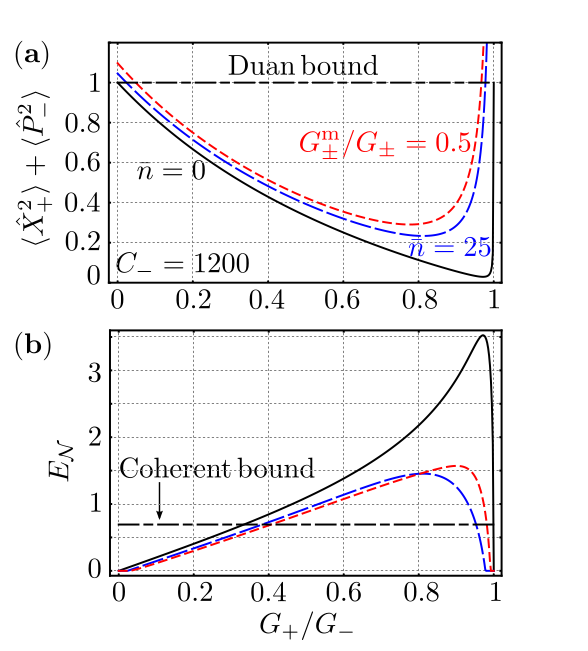
\includegraphics[width = 6 cm]{plots/plot_entanglement.png}
		\end{figure}	
	
		\column{0.5\textwidth}
		
		\begin{itemize}
			\item Duan quantity and logarithmic negativity as function of the drive asymmetry
			\item Solid curve with mechanical thermal occupation $\bar{n} = 0$ and no imperfections on effective coupling
			\item Thermal occupation and imperfections in the effective coupling lead to less entanglement
		\end{itemize}
		
	\end{columns}

\end{frame}

% Adiabatic limit IV
\begin{frame}
	
	\frametitle{Adiabatic limit}
	\framesubtitle{Entanglement}
	
	\begin{columns}
		
		\column{0.5\textwidth}
		
		\begin{figure}
			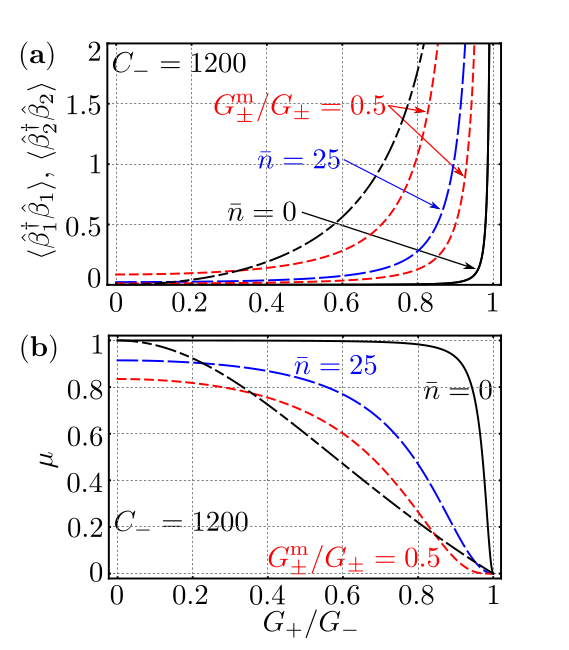
\includegraphics[width = 6 cm]{plots/plot_steady_state.png}
		\end{figure}	
		
		\column{0.5\textwidth}
		
		\begin{itemize}
			\item Steady state occupations and purity as function of the drive asymmetry
			\item Solid curve with mechanical thermal occupation $\bar{n} = 0$ and no imperfections on effective coupling
			\item Thermal occupation and imperfections in the effective coupling lead to degradation of purity
		\end{itemize}
		
	\end{columns}

\end{frame}

% Experimental observability
\begin{frame}
	
	\frametitle{Experimental observability}
	\framesubtitle{Output spectrum}
	
	\begin{itemize}
		\item Reconstructing covariance matrix is experimentally demanding
		\item Directly measuring quadratures is a hard problem
		\item Seek signature of entanglement in output spectrum
	\end{itemize}

	Spectrum as Fourier transform of expected value	
	\begin{figure}
		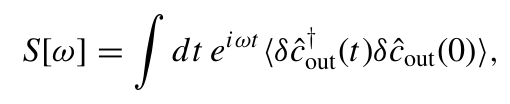
\includegraphics[width = 5.5 cm]{plots/spectrum_fourier.png}
	\end{figure}	

	being $\delta \hat{c}_{\textrm{out}} = \hat{c}_{\textrm{out}} - <\hat{c}_{\textrm{out}}>$ \\
	Spectrum can be related to the occupation of modes
	\begin{figure}
		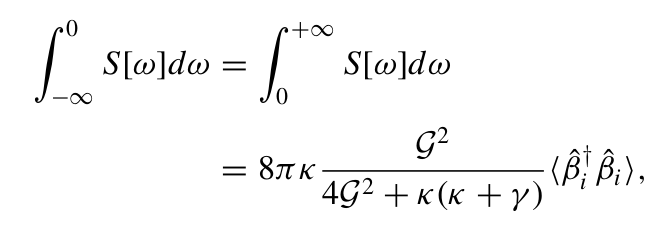
\includegraphics[width = 7 cm]{plots/spectrum.png}
	\end{figure}	

\end{frame}

% Experimental observability
\begin{frame}

\frametitle{Experimental observability}
\framesubtitle{Output spectrum}
	
	\begin{figure}
		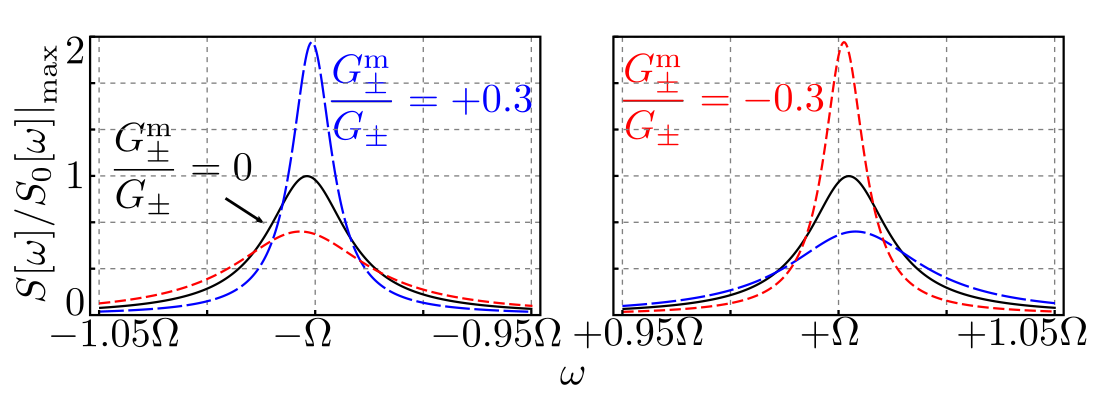
\includegraphics[width = 9 cm]{plots/plot_spectrum.png}
	\end{figure}	

	\begin{itemize}
		\item Output spectrum entered around the detunings from the cavity resonance frequency
		\item Solid black curve without imperfections
		\item Steady-state mechanical entanglement can be bounded based on a measurement of the output spectrum
		\item Experimental work realized in {\color{blue}"Stabilized entanglement of massive mechanical oscillators"}, Nature, 2018.
	\end{itemize}

\end{frame}

% Conclusions
\begin{frame}

	\frametitle{Conclusions}
	
	\begin{enumerate}
		\item Three-mode optomechanical system such as the steady state includes highly pure and highly entangled two-mode squeezed state is built.
		\item Ways of describing both entanglement and purity are described as function of the drive asymmetry.
		\item Problem of unequal single-photon optomechanical couplings solved by using four-tone driving scheme.
		\item Proposal implementable for existing technology.
	\end{enumerate}
		
\end{frame}

% Conclusions
\begin{frame}
	
	\frametitle{Thank you!}
		
	\begin{figure}
		
\includegraphics[width = 3 cm]{plots/thinking2.png}
	\end{figure}

\end{frame}

% Reservoir engineering I
\begin{frame}

	\frametitle{Back up}
	\framesubtitle{Bogoliubov operators}
	
	Define the {\color{blue}Bogoliuov} mechanical modes in terms of the modes $\hat{a}, \hat{b}$
	\begin{figure}
		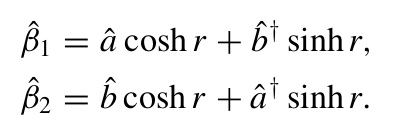
\includegraphics[width = 4.5 cm]{plots/bogoliubov_1.png}
	\end{figure}	
	
	Where r is the {\color{blue}squeezing parameter}.
	
	\vspace{0.5 cm}
	
	Work in rotating frame with respect to the Hamiltonian:
	\begin{figure}
		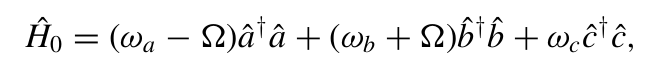
\includegraphics[width = 8 cm]{plots/hamiltonian_2.png}
	\end{figure}	
	
	where choice of detuning $\Omega$ is such that collective mechanical quadratures $\hat{X}_{\pm}$, $\hat{P}_{\pm}$ (defined later) rotate in a non-trivial way.

\end{frame}

% Back up
\begin{frame}
	
	\frametitle{Back up}
	\framesubtitle{Generate the 2-mode squeezed state}
	
	\begin{itemize}
		\item i) Two cavity modes to independently cool the Bogoliubov modes (beam splitter $\hat{\beta}^{\dagger}_{i} \hat{c}_{i}$)
		\item ii) Couple the cavity to one Bogoliubov mode ($\hat{\beta}_{1}$), and then this one to $\hat{\beta}_{2}$ through ($\hat{\beta}^{\dagger}_{1} \hat{\beta}_{2}$)
		\item iii) Couple the cavity to sum of the Bogoliubov modes , then the sum to the difference (swap interaction $\hat{\beta}^{\dagger}_{\textrm{sum}} \hat{\beta}_{\textrm{diff}}$ allows diff to cool).
		\begin{align}
		\hat{\beta}_{\textrm{sum}} = \frac{1}{\sqrt{2}}(\hat{\beta}_{1} + \hat{\beta}_{2}) \nonumber \\
		\hat{\beta}_{\textrm{diff}} = \frac{1}{\sqrt{2}}(\hat{\beta}_{1} - \hat{\beta}_{2}) \nonumber
		\end{align}
	\end{itemize}
	
	Cooling $\hat{\beta}_{\textrm{sum}}$ and $\hat{\beta}_{\textrm{diff}}$ is equivalent to cool $\hat{\beta}_{1}$ and $\hat{\beta}_{2} \; \checkmark$\\
	Direct coupling not needed, just difference in their resonance frequencies $\checkmark$

\end{frame}

% Back up
\begin{frame}
	
	\frametitle{Back up}
	\framesubtitle{4-tone driving}
	
	Where we demand the driving strengths of the 4-tone driving are "matched" as
	\begin{equation}
		{\color{blue} \frac{\bar{c}_{1\pm}}{\bar{c}_{2\pm}} = \frac{g_{b}}{g_{a}}} \nonumber
	\end{equation}

	\vspace{0.5 cm}
	
	meaning, asymmetry in steady-state amplitudes is set by the asymmetry in the optomechanical couplings

\end{frame}

% Back up
\begin{frame}
	
	\frametitle{Back up}
	\framesubtitle{Effective coupling imperfections}
	
	Imperfections in the optomechanical couplings
	\begin{align}
		G_{\pm}^{m} &= \pm(g_{a} - g_{b})\bar{c}_{\pm} / 2 \qquad \textrm{2-tone driving} \nonumber\\
		G_{\pm}^{m} &= \pm(g_{a}\bar{c}_{1\pm} - g_{b}\bar{c}_{2\pm}) / 2 \qquad \textrm{4-tone driving} \nonumber
	\end{align}
	
	\vspace{0.5 cm}
	
	In the 2-tone driving case, imperfections coming from mismatch in the optomechanical couplings
	
	\vspace{0.5 cm}
		
	In th 4-tone driving case, imperfection arises from the drives not being weighted precisely according to the matching condition

\end{frame}


\end{document}